\newpage
\section{Specifica del prodotto}
In questa sezione verrà descritta in maniera macroscopica l'architettura che verrà adottata durante l'attività di Progettazione. Per semplificare la comprensione, verrà utilizzato un approccio top-down, partendo dalle linee generali, fino a giungere ad una descrizione in dettaglio delle componenti.

\subsection{Architettura generale}
Il software API Market si caratterizza dalle comuni applicazioni per l'approccio a microservizi adottato nell'implementazione. In maniera differente da un applicazione monolitica, ogni componente viene realizzato come microservizio a sè stante. L'aggregazione di questi microservizi definisce l'applicazione finale e ne realizza il comportamento definitivo. Esulando dall'approccio a microservizi, il sistema sarà realizzato al pari di una classica applicazione \textit{Client-Server}, dove il lato \textit{front-end\ped{G}} (Client) si occuperà di fornire all'utente finale l'interfaccia web su cui poter interagire, mentre il lato \textit{back-end\ped{G}} (Server) gestirà e salverà i dati, e si occuperà della gestione delle chiamate API (tramite l'opportuna componente \textit{API Gateway}). La base di dati utilizzata, si occupa della raccolta di dati sensibili dell'utenza, della gestione delle applicazioni e delle chiavi e, infine, della gestione dei dati statistici.

Il sistema verrà realizzato, per il lato back-end, tramite microservizi con interfaccia Jolie, che verranno implementati con codice \textit{Java\ped{G}} o \textit{Jolie}. Questo approccio, sebbene la tematica sia di recente sviluppo, risulta molto gettonato dalle grandi realtà che recentemente hanno deciso di affacciarsi a questa realtà (come ad esempio l'\textit{AWS\ped{G}} Service Registry \textit{Eureka}, usato dalla piattaforma Netflix).\\
Il lato front-end, invece, verrà implementato tramite le consuete tecnologie \textit{HTML5\ped{G}}, \textit{CSS3\ped{G}} e \textit{JavaScript\ped{G}}, in particolare, l'utilizzo del framework \textit{AngularJS\ped{G}} consentirà un binding in real-time per la rappresentazione delle informazioni, di fatto fornendo una single page application.
Nella realizzazione dell'API Market richiesto, verrà utilizzato il desing pattern architetturale \textbf{\textit{Model-View-Controller}}.

\begin{figure}[H]
	\centering
	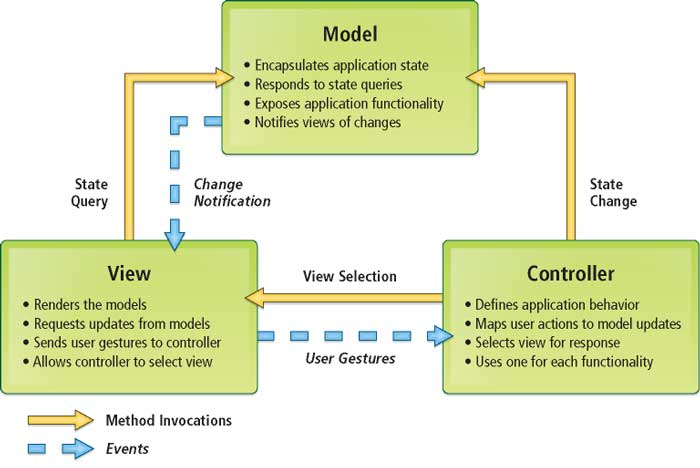
\includegraphics[width=0.7\linewidth]{IMG/MVC_pattern.jpg}
	\caption{Pattern architetturale Model View Controller}
\end{figure}

\subsubsection{Pattern architetturale Front-End}
Il pattern architetturale \textit{Model-View-Controller} (MVC) è composto di tre parti fondamentali, ed in questa sezione verranno presentate brevemente le funzionalità di ognuna. Verrà motivata, inoltre, la scelta di tale pattern da parte del team.

\begin{itemize}
	\item \textbf{Model}: rappresenta la business logic dell'applicazione, il punto di accesso ai dati, si occupa dell'interazione con essi e ne specifica le modalità di accesso. Inoltre, ha il compito di notificare le Views in caso di cambiamenti;
	\item \textbf{View}: componente che ha il compito di mostrare il contenuto dei \textit{Models} e di comunicare con i \textit{Controllers} riguardo le azioni utente sulla specifica \textit{View};
	\item \textbf{Controller}: ha il compito di definire il comportamento dell'applicazione, selezionando le corrette \textit{Views} e aggiornando i \textit{Models} in base alle azioni utente.
\end{itemize}

In fase di progettazione, il gruppo ha preso in esame diversi design pattern architetturali, ma la volontà di realizzare pagine web dinamiche e reattive, unitamente all'uso di tecnologie moderne, su tutte l'utilizzo del framework \textit{AngularJS (Angular 1)}, hanno indirizzato la scelta verso il pattern MVC. AngularJS infatti implementa tutte le componenti del pattern MVC.

\paragraph{Componente Model}
Il \textbf{Model} svolge le seguenti funzioni:
\begin{itemize}
	\item Incapsula la business logic dell'applicazione;
	
	\item Interagisce con i database, nei quali vengono salvati i dati del sistema, come API/microservizi degli utenti sviluppatori della piattaforma, transazioni e profili utenti. Le funzionalità incluse comprendono microservizi in grado di caricare, salvare, modificare e cancellare dati sui rispettivi database;
	
	\item Espone delle interfacce contenenti le funzionalità dell'applicazione;
	
	\item Notifica le rispettive \textit{Views} nel caso di cambiamenti.
\end{itemize}

\paragraph{Componente View}
La componente \textbf{View} è un'interfaccia web, ed il gruppo ha scelto di utilizzare le classiche tecnologie \textit{CSS3} e \textit{HTML5} per la struttura di base. All'utilizzo di AngularJS, per la parte View viene affiancato anche il linguaggio \textit{Javascript}. La componente View ha, quindi, lo scopo di svolgere le seguenti funzioni:

\begin{itemize}
	\item Rappresentare i dati del \textit{Model};
	
	\item Richiedere degli aggiornamenti ai rispettivi \textit{Models};
	
	\item Comunicare e inoltrare tutte le azioni utente ai relativi \textit{Controllers};
	
	\item Permettere ai \textit{Controllers} di selezionare le corrette \textit{Views}.
\end{itemize} 

\paragraph{Componente Controller}
La componente \textbf{Controller} comunica sia con la componente \textit{View} che con la componente \textit{Model}. Essa è l'unica componente a conoscere gli altri, realizzando un totale disaccopiamento tra \textit{View} e \textit{Model}. Il Controller ha il compito di svolgere le seguenti funzioni:
\begin{itemize}
	\item Definire il comportamento dell'applicazione, in particolare definendo le risposte alle azioni utente;
	
	\item Realizzare il data-binding tra le azioni utente sulle \textit{Views} e gli aggiornamenti di stato dei relativi \textit{Models};
	
	\item Selezionare le corrette Views da visualizzare all'utente;
	
	\item Ogni \textit{Controller} è associato ad una singola funzionalità.
\end{itemize}

\subsubsection{Pattern architetturale Back-End}
Molti dei microservizi pensati per la parte di comunicazione con i database sono stati progettati per essere relizzati seguendo il design pattern \textbf{\textit{Aggregator Microservices}}. 
\begin{figure}[H]
	\centering
	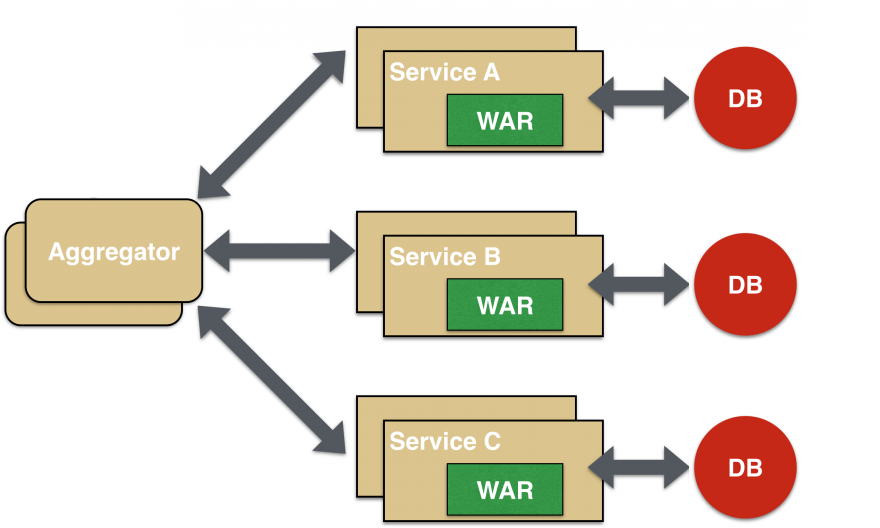
\includegraphics
	[width=0.7\linewidth]
	{IMG/microservices-aggregator}
	\caption{Aggregator Microservices design pattern}
\end{figure}
Questo design pattern si compone di un \textit{aggregatore}, ovvero un microservizio in grado di collezionare i dati che gli vengono forniti da diversi microservizi, per poi renderli fruibili all'utente, tramite la componente \textit{View}. Utilizzando un design pattern a microservizi è necessario che le varie componenti siano indipendenti tra loro e, quindi, che lo siano anche i relativi database. Tutti i microservizi contenuti in un package, sono indipendenti da microservizi contenuti in altri package, ed ogni microservizio opera sul proprio database associato.

\subsubsection{Pattern architetturale API Gateway}
Il design pattern architetturale scelto per parte dell'implementazione dell'API Gateway è il design pattern \textbf{\textit{Chain Microservices}}. Questo tipo di pattern consiste di una sequenza di azioni prestabilite, innescate da una richiesta \textit{HTTP\ped{G}}. 
\begin{figure}[H]
	\centering
	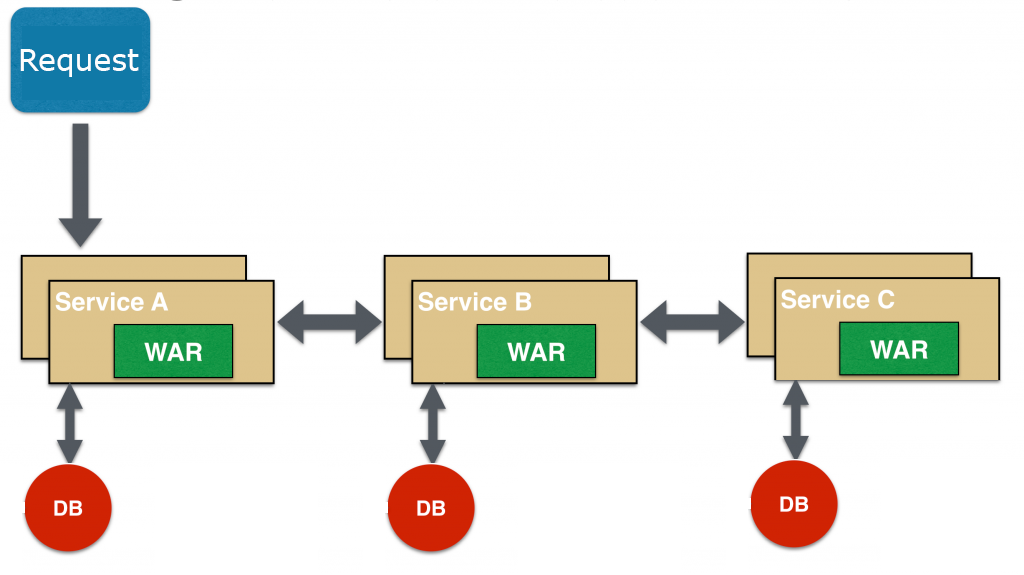
\includegraphics
	[width=0.7\linewidth]
	{IMG/microservices-chain}
	\caption{Chain Microservices design pattern}
\end{figure}
Ogni servizio non può intraprendere la propria esecuzione se non è terminato il servizio precedente. Un punto critico di questa scelta è la lunghezza della catena. L'API Gateway è progettato per elaborare una richiesta e ritornare una risposta al chiamante, trattandosi, dunque, di richieste sincrone. Una catena troppo lunga crea una tempo di attesa non indifferente per il client, considerando che bisogna valutare anche il tempo impiegato dal microservizio target della chiamata all'API Gateway.


